% !Mode:: "TeX:UTF-8" 



\setcounter{tocdepth}{1}                % 目录深度——\section
\setcounter{secnumdepth}{0}             % 编码深度——\chapter

\titleformat{\chapter}{\huge}{}{1em}{}

\BiChapter{第二章}{Figures, Tables and Equations}

除非另外说明,在下列习题中,都使用表2.1中的器件数据,如果涉及到$V_{DD}$,则$V_{DD}=3V$。

\BiSection{2.1}{Figures}

\fancyhead[R]{本题2.1由QC.Z完成}

$\frac{W}{L}=\frac{50}{0.5}$,假设$|V_{DS}|=3V$,当$|V_{GS}|$从0上升到3V时,画出NFET和PFET的漏电流随$V_{GS}$变化曲线。




解:

(1)对于NFET:
	
当$V_X<V_{TH}$时,见图1,漏电流$I_D\cong0A$
	\begin{figure}[H] %H为当前位置,!htb为忽略美学标准,htbp为浮动图形
	\centering %图片居中
	\begin{minipage}{\linewidth}
		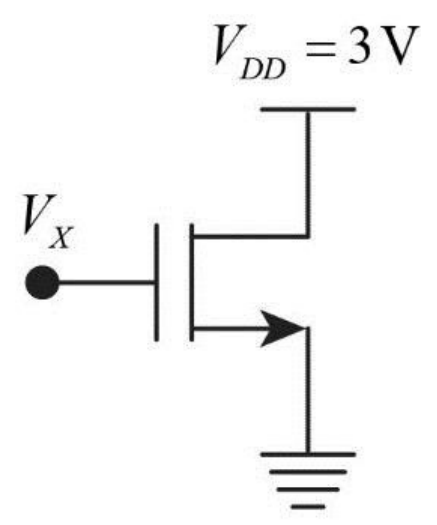
\includegraphics{2.1-1}
	\end{minipage}
	\caption*{图1:NFET的示意图} %最终文档中希望显示的图片标题
	\label{fig1} %用于文内引用的标签
\end{figure}

$C_{ox}=\frac{\epsilon_{ox}}{T_{ox}}=\frac{3.9 \times 8.854 \times 10^{-12}\frac{F}{m}}{9 \times 10^{-9}m}=3.837 \times 10^{-3}\frac{F}{m^2}$

当$V_X>V_{TH}$时,$I_D=\frac{1}{2}\mu_nC_{ox}\frac{W}{L_{eff}}(V_{GS}-V_{TH})^2(1+\lambda V_{DS})=\frac{1}{2}\mu_nC_{ox}\frac{W}{0.5\mu m-2L_D}(V_{X}-V_{TH})^2(1+\lambda V_{DS})=(12.8\frac{mA}{V^2})(V_X-0.7V)^2$

\color{blue}{
	\{
	$V_{TH},\mu_n,\lambda,L_D\text{见教材表2.1中,单位换算}\frac{A \cdot s}{V}=F$
	\begin{figure}[H] %H为当前位置,!htb为忽略美学标准,htbp为浮动图形
		\begin{minipage}{\linewidth}
		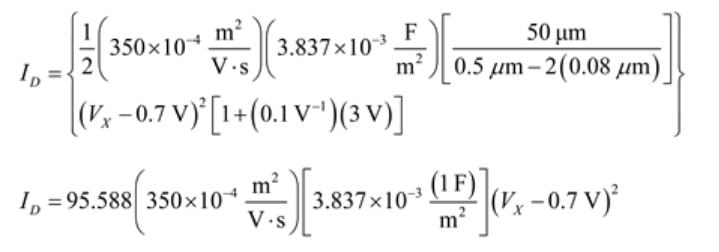
\includegraphics{2.1-2}
		\end{minipage}
		\label{fig02} %用于文内引用的标签
	\end{figure}
	
	\begin{figure}[H] %H为当前位置,!htb为忽略美学标准,htbp为浮动图形
	\begin{minipage}{\linewidth}
		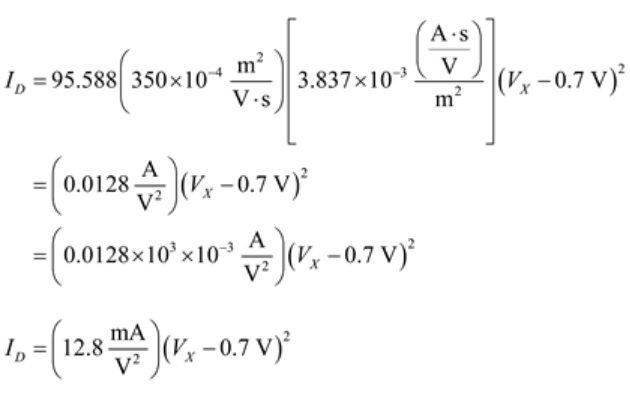
\includegraphics{2.1-3}
	\end{minipage}
	\label{fig03} %用于文内引用的标签
\end{figure}
\}
	
}

\color{black}{
	
	\begin{figure}[H] %H为当前位置,!htb为忽略美学标准,htbp为浮动图形
		\centering %图片居中
		\begin{minipage}{\linewidth}
		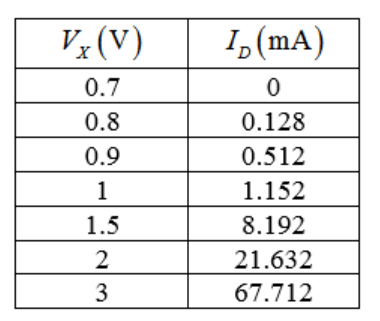
\includegraphics{2.1-4}
	\end{minipage}
		\caption*{表1} %最终文档中希望显示的图片标题
		\label{tab1} %用于文内引用的标签
	\end{figure}
	\begin{figure}[H] %H为当前位置,!htb为忽略美学标准,htbp为浮动图形
		\centering %图片居中
			\begin{minipage}{\linewidth}
		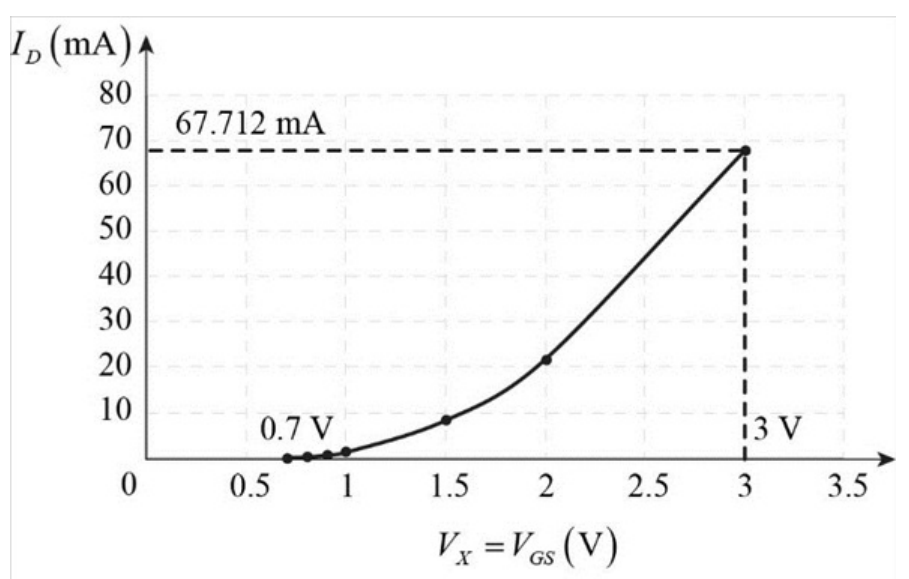
\includegraphics{2.1-5}
	\end{minipage}
		\caption*{图2} %最终文档中希望显示的图片标题
		\label{fig2} %用于文内引用的标签
	\end{figure}
	
	
	
	(2)对于PFET:
	
	当$V_X<V_{TH}$时,见图3,漏电流$I_D\cong0A$
	\begin{figure}[H] %H为当前位置,!htb为忽略美学标准,htbp为浮动图形
		\centering %图片居中
		\begin{minipage}{\linewidth}
		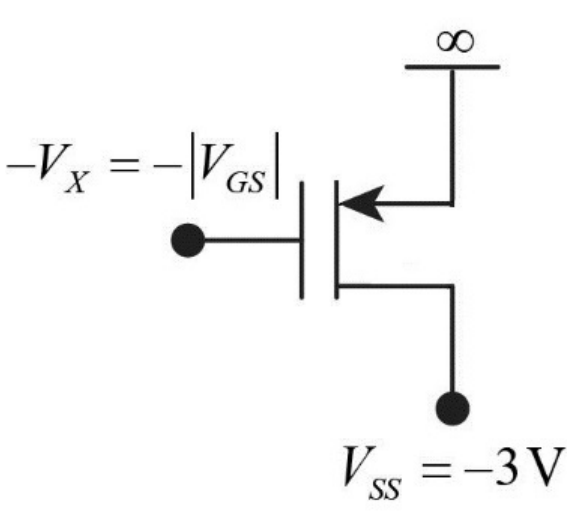
\includegraphics{2.1-6}
	\end{minipage}
		\caption*{图3:PFET的示意图} %最终文档中希望显示的图片标题
		\label{fig3} %用于文内引用的标签
	\end{figure}
	
	当$V_X>V_{TH}\text{或}|V_{GS}|>V_{TH}$时,$I_D=\frac{1}{2}\mu_pC_{ox}\frac{W}{0.5\mu m-2L_D}(V_{X}-V_{TH})^2(1+\lambda V_{DS})=(4.8\frac{mA}{V^2})(V_X-0.8V)^2$
}
\color{blue}{
	\{
	$V_{TH},\mu_p,\lambda,L_D\text{见教材表2.1中,单位换算}\frac{A \cdot s}{V}=F$
	\begin{figure}[H] %H为当前位置,!htb为忽略美学标准,htbp为浮动图形
	\begin{minipage}{\linewidth}
		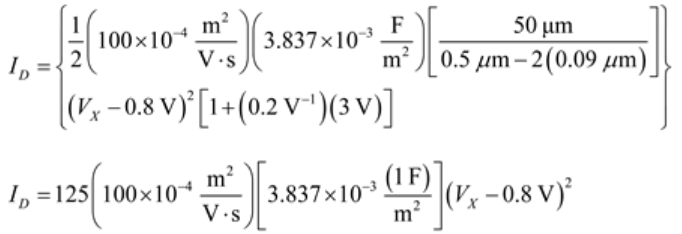
\includegraphics{2.1-7}
	\end{minipage}
	\label{fig07} %用于文内引用的标签
\end{figure}

\begin{figure}[H] %H为当前位置,!htb为忽略美学标准,htbp为浮动图形
	\begin{minipage}{\linewidth}
		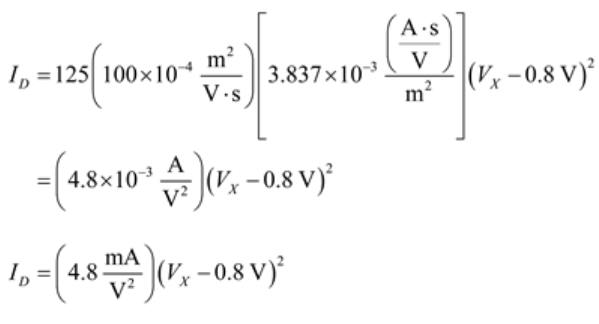
\includegraphics{2.1-8}
	\end{minipage}
	\label{fig08} %用于文内引用的标签
\end{figure}
	\}
	
	\begin{figure}[H] %H为当前位置,!htb为忽略美学标准,htbp为浮动图形
	\centering %图片居中
	\begin{minipage}{\linewidth}
		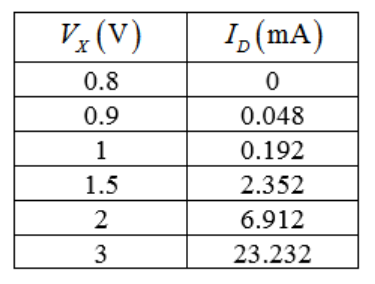
\includegraphics{2.1-9}
	\end{minipage}
	\caption*{表2} %最终文档中希望显示的图片标题
	\label{tab2} %用于文内引用的标签
\end{figure}
\begin{figure}[H] %H为当前位置,!htb为忽略美学标准,htbp为浮动图形
	\centering %图片居中
	\begin{minipage}{\linewidth}
		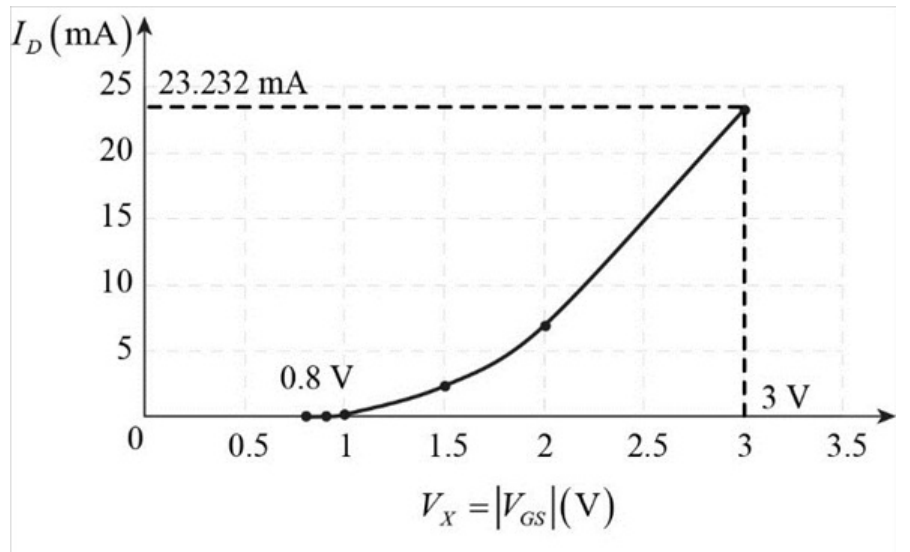
\includegraphics{2.1-10}
	\end{minipage}
	\caption*{图4} %最终文档中希望显示的图片标题
	\label{fig4} %用于文内引用的标签
\end{figure}
	
}

\color{black}{}